\chapter{Technical Approach}
In this chapter, the approaches employed in this work are explained.
Firstly, confronted with the limitations of concrete dropout, an adapted version of concrete dropout is proposed called multiple dropout (multi-drop).
Secondly, a modified architecture of ResNet50 is introduced in order to incorporate different inference techniques for BNN with this powerful feature extraction network.
Thirdly, a pipeline which combines BNN and CRF is presented.
Thereby, The CRF works as a post-processor to capture the relationship between random variables.
Last but not least, the approach combining aforementioned techniques for continuous learning is introduced.


\section{Multiple dropout}
Based on Fig.\ref{fig:dropout} and the expression of the approximate distribution in equation \ref{appro_dist_form}, only one probability of Bernoulli distributed random variable for each layer is chosen, therefore random vector $\bld p_i = [p_i]^{D_{i-1}}$ for $i$-th layer, which stacks same value into a vector. %\todo{this sentence I do not understand...is there something missing?}
While the dropout regularization term pushes the probability of Bernoulli to 0.5 to maximize its entropy, the expected likelihood term tries to increase the probability since a decreasing probability will lead to a different model with lower capacity and thus lower performance.
Thus, an equilibrium state between them should be achieved in training.
With the concrete dropout introduced above, this approach can be extended for each hidden unit instead of each layer(cf. Fig.\ref{fig:multi-drop}), which results in the random vector $\bld p_i = [p_i^k]_{k=1}^{D_{i-1}}$.
The difference between multiple dropout and concrete dropout can be easily seen by comparing the figures Fig.~\ref{fig:multi-drop} and Fig.~\ref{fig:dropout_inference}.
While the first term in the gradients computation stays the same, the second term should be modified to:
\begin{equation} 
\begin{aligned}\label{KL_grad_multi}
\frac{\partial KL(q_{\theta}(\bld \omega)||p(\bld \omega))}{\partial \theta} 
&\approx \frac{\partial \sum_{i=1}^{L}\lambda||\bld M_{i}||^{2}- \beta \mathcal H(\bld p_{i})}{\partial \theta}  \\
&= \frac{\partial}{\partial \theta} \big( \sum_{i=1}^{L}\lambda||\bld M_{i}||^{2}- \beta \sum_{k=1}^{D_{i-1}}(-p_i^k\text{log}p_i^k - (1-p_i^k)\text{log}(1-p_i^k))\big)
\end{aligned}
\end{equation}  

The reasons for multi-drop are as following:
\begin{itemize}
	\item to increase flexibility in tuning variational parameters. The tunability of the parameter of the Bernoulli random variable in the likelihood term is low since there is only a single parameter controlling the entire layer. As observed in the experiments(cf. Fig.\ref{fig:cdp_dropout2}), these parameters are always increased for each layer.\todo[inline]{in the sentence before you talk about one single parameter and in this sentence it is plural. is this correct?} The reason for this is probably that reducing it would lead to low capacity and thus low likelihood. 
	
	\item the solution space of concrete dropout should be a subset of the solution space of multi-drop if all of them are reachable. Because if it is optimal to assign the same probability for each hidden unit, this can be recovered in training with the multi-drop. Otherwise, other optimal solutions of assigning different probabilities to different hidden units could be considered.
	
	\item multi-drop can extend the flexibility and diversity of the dropout approximate distribution family by adding more parameters. Hence the truth posterior can be approximated better by the approximate posterior.
	
\end{itemize}

\begin{figure}
	\begin{center}
		\centering
		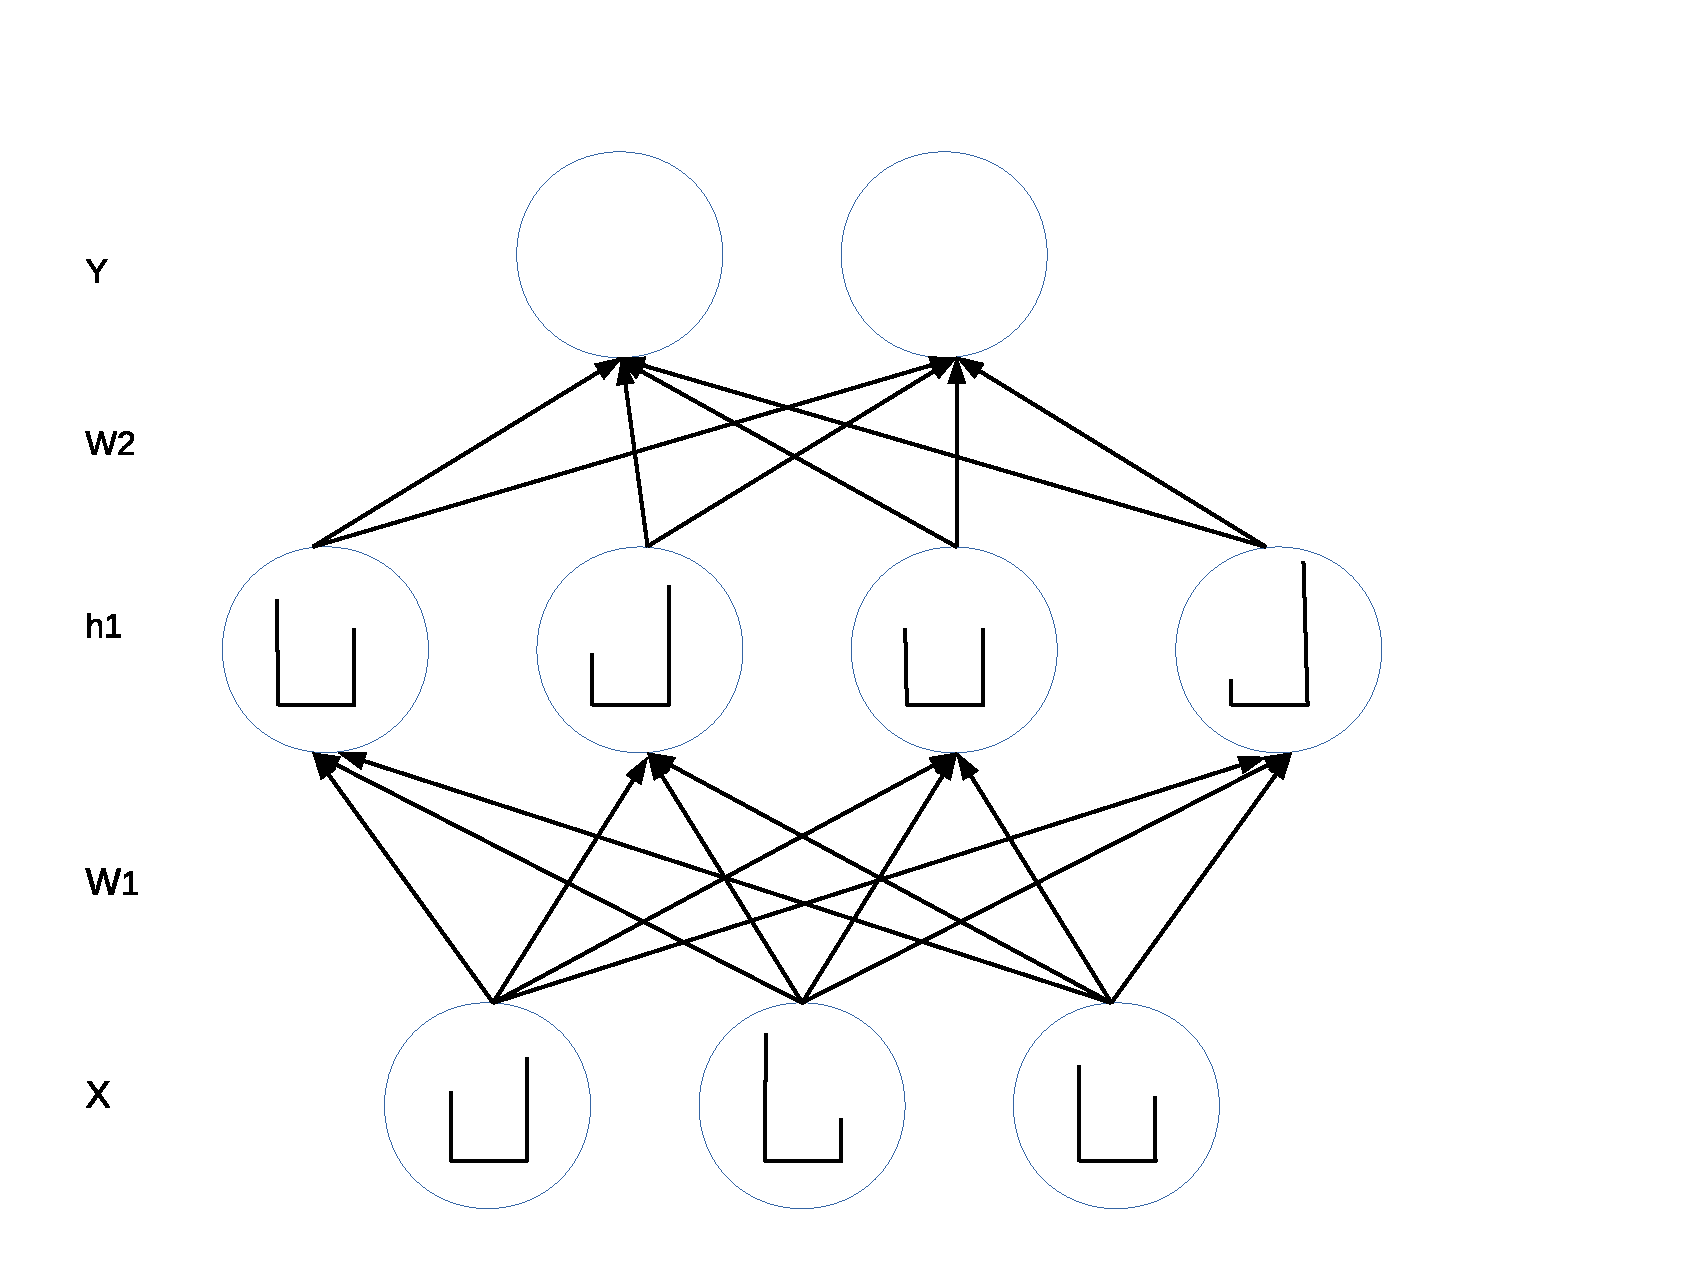
\includegraphics[width=11cm]{multi-drop}
		\caption{Different dropout rates for different hidden units in multi-drop.}		
		\label{fig:multi-drop}
	\end{center}
\end{figure}

\begin{figure}[H]
	\begin{center}
		\includegraphics[height=4cm, width=11cm]{cdp_dropout1}	
		\caption{Changes of keep probability of the first two concrete dropout layers during training.}
		\label{fig:cdp_dropout1}
	\end{center}
\end{figure}
\todo[inline]{this figure is not referenced/used}
\begin{figure}[H]
	\begin{center}
		\includegraphics[height=4cm, width=11cm]{cdp_dropout2}	
		\label{fig:cdp_dropout2}
		\caption{Changes of keep probability of the last two concrete dropout layers during training.}
	\end{center}
\end{figure}



\section{Modified network architecture}
After introducing dropout and concrete dropout variational inference, in this subsection the modified network architecture is described.
As already mentioned, the fundamental task in this work is object classification.
Thus, due to its strong ability to learn powerful representation for images a ResNet50\cite{he2016deep} pre-trained on ImageNet as backbone for fine-tuning is selected. 
However, there is no dropout in the original version of this network.
In order to employ dropout variational inference for a reliable uncertainty estimation, the dropout concept should be inserted into the network.
In this work, three fully connected layers with 1024 hidden units are added before the output layer -- whose dimension needs to be set to the number of classes -- which are initialized from scratch. 
Next, a concrete dropout at flatten layer is added, and at the three new fully connected layers, respectively.
There are three reasons why the network is modified this way:
\begin{itemize}
	\item By inserting dropout in pre-trained layers, the pre-trained features will get destroyed. Since the major part of the network is initialized with pre-trained weights, hence this would lead to a significant drop of performance after fine-tuning.
	\item According to the suggestions from \cite{srivastava2014dropout}, insertion of dropout reduces the capacity of the model and thus a model with dropout should have larger capacity than one without dropout. Therefore three additional fully connected layers are added to ensure that the model possesses a large enough model capacity.
	\item As introduced in previous sub-sections, weights are a major part of variational parameters. Therefore, more weights can enhance the flexibility and capacity of the approximate distribution family, which improves the quality of approximation.  
\end{itemize}

Fig.\ref{fig:modified_net} shows the sketch of the modified network architecture.
The major part of the network without dropout can be interpreted as deterministic feature extractor.
Following this, the four layers with dropout work as a probabilistic classifier.
These four layers include one flatten layer with 2048 hidden units, and three fully connected layer with 1000 hidden units each.
At the end, an output layer with the size of number of categories is appended.
The version of dropout inserted can be normal dropout, concrete dropout or multiple dropout.
In this report, only results of concrete dropout and multiple dropout are presented since normal dropout significantly underperforms.

During training, these two parts are trained together in order to achieve a better balance between uncertainty estimation and accuracy.
As known to all, freezing the feature extraction part can lead to worse performance, but it can also reduce the influence on predictive uncertainty from aleatoric uncertainty.
To investigate this effect, an ablation study is conducted shown in experiment part.
In testing, possible parameters according to posterior distribution have to be marginalized.
Layers with dropout should be turned on, sampled and run multiple times to perform Monte Carlo integration to approximate predictive distribution.
The reduction of run time during testing can be achieved by different techniques, such as parallel computing or distillation.
But this surpass the scope of this work.
\begin{figure}[H]
	\begin{center}
		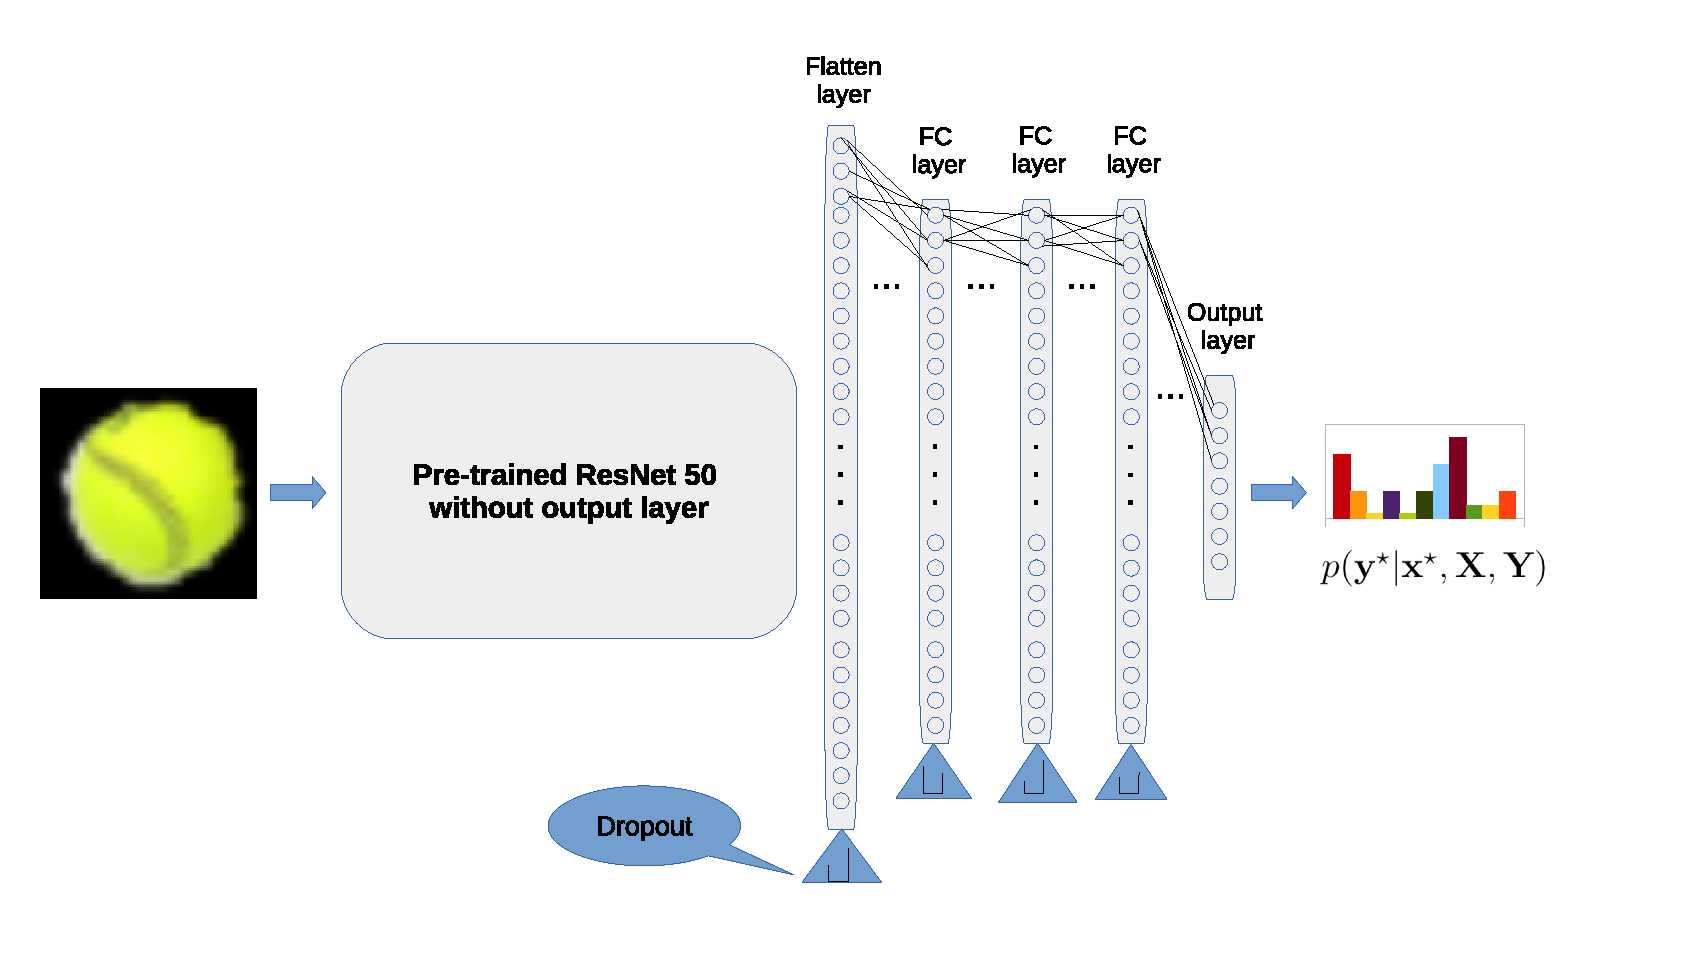
\includegraphics[height=8.5cm, width=15.5cm]{m_network}
		\caption{Modified network architecture of ResNet50.}		
		\label{fig:modified_net}
	\end{center}
\end{figure}

\section{Combination with CRF}\label{com_crf}
After employing Bayesian neural network, the model can provide more reliable uncertainty estimation in a probabilistic manner.
In other words, the predicted probability distribution contains more valuable information than before.
In order to make use of this information another probabilistic model is applied.
The idea is to combine the output from BNN and relationships between the objects in a scene via a CRF.
In detail, the output distribution from BNN is used as unary feature and a binary co-occurrence matrix for pairwise feature (introduced in \ref{crf_def}). 
Fig.\ref{fig:combined_crf} demonstrates the flow chart how BNN and CRF are combined together.
As can be seen, objects in one scene are firstly fed into BNN and their output distributions are fed into the CRF as unary feature for each node.
In the scene, their contextual relationship is represented by the binary co-occurrence matrix which is forwarded to the CRF as pairwise feature.
Then loopy belief propagation is applied to infer the marginal distribution of each node.

One key factor in this case is that the pairwise feature is required to be designed by hand.
The choice and design of it have significant impact on the improvement achieved by CRF.
The information brought by pairwise feature should be complementary instead of contradictory to that of unary feature.
Once this point is fulfilled, the more information the unary feature has, the more improvement CRF can achieve. \todo[inline]{isn't the pairwise feature meant in this sentence?}

One thing worth noting, in experiment part, this approach is tested only on the T-LESS dataset, since constructing scenes for objects in the WRGBD dataset is non-trivial.
The reason therefore is that most objects there have not only similar appearances but also similar contexts.
Therefore it is hard to disambiguate miss-classification by incorporating their contextual information.
\begin{figure}[H]
	\begin{center}
		\includegraphics[height=8cm, width=15cm]{combined_crf}
		\caption{Combination of BNN and CRF.}		
		\label{fig:combined_crf}
	\end{center}
\end{figure}
\section{Approach for continuous learning}
With a reliable uncertainty estimation, one of our goals is to enable the classifier or robot to learn continuously.
The classifier should be introspective and express the confidence about its predictions.
It is common that the test data in real environment does not have exactly the same distribution as the training set, which induces a significant performance drop.
In this situation, the classifier is expected to adapt itself to the real environment by fine-tuning itself with as little manual effort for the user as possible. 

This idea is visualized in Fig.\ref{fig:con_learn}.
The initialization phase includes the training of the model with an easily obtainable dataset, which can be a public or synthetic dataset.
Before deploying to the real environment, there is an adaptation phase which makes use of the aforementioned techniques.
In this phase, the classifier should be able to adapt itself to the objects in the real environment by fine-tuning with the dataset collected. 
The annotations for the collected dataset are generated automatically by the initial network and manually by the user.
In order to prevent a high amount of miss-classified training data for fine-tuning, only high confident predictions are used for the automatic labeling.
Therefore, a reliable uncertainty estimation is essential.
If the relationship between objects in real environment is complementary to the discriminative classifier and can be encoded well, the CRF can be employed to capture the relationship to further improve the performance (cf. section \ref{com_crf}).
After that, the classifier is deployed to the test data in the real environment.
In the experiment part, this approach is evaluated on both UniHB(WRGBD) and T-LESS(synthetic T-LESS) data.
\begin{figure}[H]
	\begin{center}
		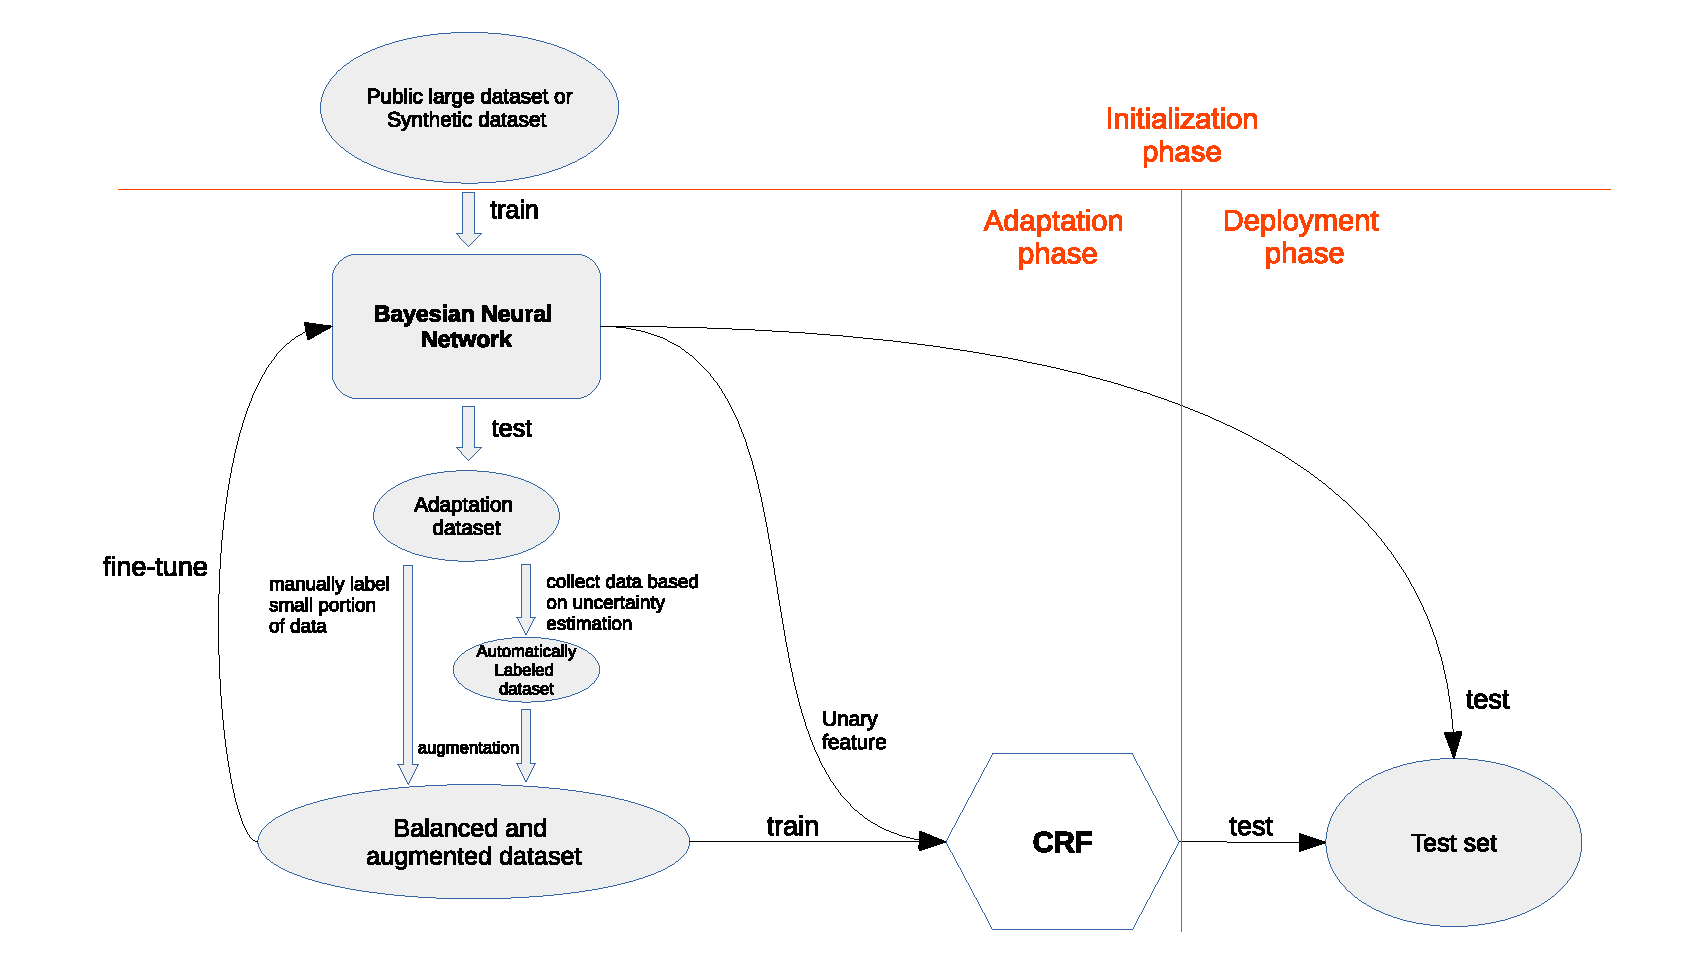
\includegraphics[height=10cm, width=16.5cm]{con_learn}
		\caption{Approach for continuous learning.}		
		\label{fig:con_learn}
	\end{center}
\end{figure}
